\documentclass[journal]{IEEEtran}
\usepackage{blindtext}
\usepackage{graphicx}
\usepackage{algorithm2e}
\usepackage{amsmath}
\usepackage{amsfonts}
\usepackage{graphicx}
\usepackage{tabularx}
\usepackage{float}
\usepackage{bm}


\begin{document}

\title{GPU-Accelerated Parallelization of Edge-Based Motion Detection Algorithms with the NVIDIA CUDA Framework}

\author{
	Emilio Del Vecchio, Kevin Lin, Senthil Natarajan\\
	Department of Electrical and Computer Engineering, Rice University, Houston, TX\\
	\{edd5, kevinlin, ssn3\}@rice.edu
}

\maketitle


\begin{abstract}
GPUs provide a powerful platform for parallel computations on large data inputs, namely images. In this paper, we explore a GPU-based implementation of a simplified adaptation of existing edge detection algorithms fast enough to operate on frames of a continuous video stream in real-time. We also demonstrate practical applications of edge detection, including an edge-based method for motion detection estimation. Finally, we demonstrate the speedups of over 2x we achieve with GPU parallelism, as compared to a reference serial CPU-based implementation.
\end{abstract}


\section{Introduction}
Graphics processing units (GPUs) are rapidly gaining popularity as a platform for parallelized computations on massive sets of data. Since much of the computations in image processing and computer vision are easily parallelized, graphics operations on GPUs achieve significant speedups compared to those done on their serial, CPU counterparts. Further, SDKs like the NVIDIA CUDA framework provide developers easy APIs to take advantage of the parallel computing power of GPUs. We take full advantage of the computational benefits of GPUs by implementing edge detection and motion detection algorithms in CUDA C.

\subsection{GPU Computation and the NVIDIA CUDA Framework}
Formally, NVIDIA CUDA is a parallel computing platform and programming model that exposes familiar C-based APIs for parallelized computations. CUDA is NVIDIA's platform for general-purpose computing on graphics processing units (commonly, GPGPU or GP$^2$U), or the use of a GPU for computations traditionally handled by the CPU. Generally, GPGPU is used to exploit the improved multithreaded performance and raw floating-point computational ability of GPUs over CPUs. For example, on modern hardware, an NVIDIA GeForce GTX 970 (1664 CUDA cores) exhibits peak single-precision floating point performance of nearly 3500 GFLOPS (floating-point operations per second), while an Intel Core i7 4790K (8C, 16T) achieves 100 GFLOPS. Our goal is to demonstrate the performance of GPU computing by solving a handful of existing problems in computer vision with CUDA: namely, edge detection and motion detection.


\section{Edge Detection Algorithm}
Edge detection is the process of determining the locations of boundaries that separate objects, or sections of objects, in an image. This edge data simplifies the features of an image to only its basic outlines, which makes it a convenient input for many other problems in computer vision, including motion detection and tracking, object classification, three-dimensional reconstruction, and others. The edge detection algorithm we present is composed of three stages:
\begin{enumerate}
	\item Reduce the amount of high-frequency noise from the image using a two-dimensional low pass filter.
	\item Determine the two-dimensional gradient of the filtered image by applying partial derivatives in both the horizontal and vertical directions.
	\item Classify edges by suppressing surrounding pixels in the gradient direction whose magnitude is lesser, and applying selective thresholding to a limited apron around each selected pixel.
\end{enumerate}
Edges correspond to the points on the image that exhibit a high gradient magnitude. The edge data from our algorithm is then used as input to our motion detection algorithm.

\subsection{Separable Convolution}
The filtering necessary in steps (1) and (2) from our algorithm above involve the convolution of a two-dimensional image and a two-dimensional kernel filter of constant width and height. A na\"{\i}ve implementation of two-dimensional convolution would require a double sum across the kernel and image for each individual pixel:
\begin{equation}
	\label{2d-naive-convolution}
	y[m, n] = x[m, n] * h[m, n] = \sum_{i = -\infty}^{\infty} \sum_{j = -\infty}^{\infty} h[i, j] x[m - i, n - j]
\end{equation}
For an image of size $M$ x $N$ and kernel of size $k$, a direct implementation would require $O(MNk^2)$ time, which is infeasible for a real-time implementation. Instead, it is possible to exploit the separable property of certain convolution matrices $h$, e.g. that $h$ can be represented as the product of two one-dimensional matrices $h_1$ and $h_2$. This effectively reduces our two-dimensional convolution of \eqref{2d-naive-convolution} to two separate instances of one-dimensional convolution:
$$y[m, n] = h_1[n] * (h_2[m] * x[m, n])$$
which is implemented as
$$y[m, n] = \sum_{i = -\infty}^{\infty}h_1[i] \sum_{j = -\infty}^{\infty}h_2[j] x[m - i, n - j]$$
For the same $M$ x $N$ input and square kernel of size $k$, a separable implementation reduces the computational complexity to $O(MNk)$. By comparison, an implementation using the FFT would cost $O(MN\log{MN})$. In practice, consider the following results\footnote{Results were obtained by measuring the execution time of a MATLAB script on an Intel Core i7 4790K @ 4.7 GHz.} for a convolution of a $3$ x $3$ kernel with an image of size $2500$ x $2500$:
\begin{table}[H]
	\small
	\centering
	\caption{Comparison of Computational Complexity of Different Convolution Implementation Algorithms}
	\label{convolution-complexity-comparison}
	\begin{tabular}{llll}
	 & Complexity & Execution time (s) \\
	 Direct convolution & $O(MNk^2)$ & $3$ \\
	 Separated convolution & $O(MNk)$ & $3$ \\
	 FFT & $O(MN\log{MN})$ & $3$
	\end{tabular}
\end{table}
As detailed in later sections, we take advantage of the fast computational complexity of separable convolution in our implementation, as all of the filters we apply are separable into one-dimensional matrices.


\subsection{Noise Elimination: Two-Dimensional Gaussian Filtering}
The first task in our edge detection algorithm is denoising the input in order to reduce the amount of high-frequency content in the image by as much as possible without destroying critical information points in the image (e.g. the real edges). We filter out high-frequency noise so that random noise is not mistakenly interpreted as an edge, as edges correspond to points in the image where the gradient has an above-threshold magnitude. \par
For example, consider the $5312$ x $2988$ pixel image (taken at a high ISO to deliberately introduce noise) of Figure \ref{noisy-image} and a plot of its grayscale intensity versus the image's spatial dimensions in Figure \ref{noisy-image-mesh}. It is clear from the mesh that there is much high-frequency noise, which can be removed with a low-pass filter.
\begin{figure}[H]
	\centering
	\includegraphics[width=0.45\textwidth]{noisy_image.jpg}
	\caption{Unfiltered noisy image}
    \label{noisy-image}
\end{figure}
\begin{figure}[h]
	\centering
	\includegraphics[width=0.45\textwidth]{noisy_image_mesh.jpg}
	\caption{Grayscale intensity of unfiltered noisy image at each pixel}
    \label{noisy-image-mesh}
\end{figure}
\begin{figure}[h]
	\centering
	\includegraphics[width=0.45\textwidth]{fft_noisy_image.jpg}
	\caption{FFT magnitude of unfiltered noisy image at each pixel (log scale)}
    \label{noisy-image-fft}
\end{figure}
To low-pass filter our image, we apply a discrete Gaussian filter. Generally, a Gaussian blur kernel of size $2n + 1$ x $2n + 1$ ($\forall n \in \mathbb{Z}^+$, and with parameter $\sigma$) is given by
$$h[i, j] = \frac{1}{2\pi \sigma^2}e^{-\frac{(i - k - 1)^2 + (j - k - 1)^2}{2\sigma^2}}$$
Our implementation of Gaussian filtering uses the constant-sized ($k = 3$), constant-$\sigma$ kernel
\[
h[i, j] = \frac{1}{16}
\begin{bmatrix}
	1 & 2 & 1 \\
	2 & 4 & 2 \\
	1 & 2 & 1
\end{bmatrix}
\]
This kernel is implemented separably as
\[
h[i, j] = \frac{1}{16}
\begin{bmatrix}
	1 & 2 & 1
\end{bmatrix}
*
\begin{bmatrix}
	1 \\ 2 \\ 1
\end{bmatrix}
\] \par
Applying a Gaussian filter with parameters $k = 5$ and $\sigma = 5$ to the above image significantly denoises the image without sacrificing edge precision, which can be seen from the spatial intensity plot in Figure \ref{filtered-noisy-image-mesh}.
\begin{figure}[H]
	\centering
	\includegraphics[width=0.45\textwidth]{filtered_noisy_image.jpg}
	\caption{Gaussian-filtered noisy image with parameters $k = 3$ and $\sigma = 5$}
    \label{filtered-noisy-image}
\end{figure}
\begin{figure}[h]
	\centering
	\includegraphics[width=0.45\textwidth]{filtered_noisy_image_mesh.jpg}
	\caption{Grayscale intensity of Gaussian-filtered noisy image at each pixel}
    \label{filtered-noisy-image-mesh}
\end{figure}
\begin{figure}[h]
	\centering
	\includegraphics[width=0.45\textwidth]{fft_filtered_noisy_image.jpg}
	\caption{FFT magnitude of Gaussian-filtered noisy image at each pixel (log scale)}
    \label{filtered-noisy-image-fft}
\end{figure}

\subsection{Gradient Computation: The Sobel Operator}
Edges in the image correspond to pixel locations at which there is a rapid change in intensity with respect to the image's spatial dimensions. Thus, edge pixels are defined as those whose gradient magnitude $||\boldsymbol{G}||$ is maximized along the gradient direction $\theta_G$.
\begin{equation}
	\label{gradient-magnitude}
	||\boldsymbol{G}_{i,j}|| = \sqrt{G_x^2 + G_y^2}
\end{equation}
\begin{equation}
	\label{gradient-angle}
	\theta_G = \arctan{\frac{G_y}{G_x}}
\end{equation}
where $G_x$ and $G_y$ are the values of the partial derivatives along the $x$ and $y$ directions, respectively, at the pixel located at $(i, j)$ of the image $A$.
$$G_x = \frac{\partial \boldsymbol{A}}{\partial x}\Bigr|_{\substack{(x, y) = (i, j)}}$$
$$G_y = \frac{\partial \boldsymbol{A}}{\partial y}\Bigr|_{\substack{(x, y) = (i, j)}}$$
\par A variety of different discrete differentiation operators exist to approximate the gradient of the image. The operator we choose in our implementation is the Sobel operator.
\[
\boldsymbol{G_x} =
\begin{bmatrix}
	-1 & 0 & 1 \\
	-2 & 0 & 2 \\
	-1 & 0 & 1
\end{bmatrix} * \boldsymbol{A}
\]
\[
\boldsymbol{G_y} =
\begin{bmatrix}
	-1 & -2 & -1 \\
	0 & 0 & 0 \\
	1 & 2 & 1
\end{bmatrix} * \boldsymbol{A}
\]
Like our Gaussian kernel, the Sobel operator (in both the $x$ and $y$ directions) is separable:
\[
\boldsymbol{G_x} =
\begin{bmatrix}
	1 \\
	2 \\
	1
\end{bmatrix} * 
(\begin{bmatrix}
	1 & 0 & -1
\end{bmatrix} * \boldsymbol{A})
\]
\[
\boldsymbol{G_y} =
\begin{bmatrix}
	1 \\
	0 \\
	-1
\end{bmatrix} * 
(\begin{bmatrix}
	1 & 2 & 1
\end{bmatrix} * \boldsymbol{A})
\]
\par Thus, we perform two separable convolutions with the separated Sobel filter on the Gaussian-filtered image to obtain gradients in the horizontal and vertical directions, and determine the magnitude and angle matrices $\boldsymbol{G}$ and $\boldsymbol{\theta}$ from equations \eqref{gradient-magnitude} and \eqref{gradient-angle}.
\begin{figure}[h]
	\centering
	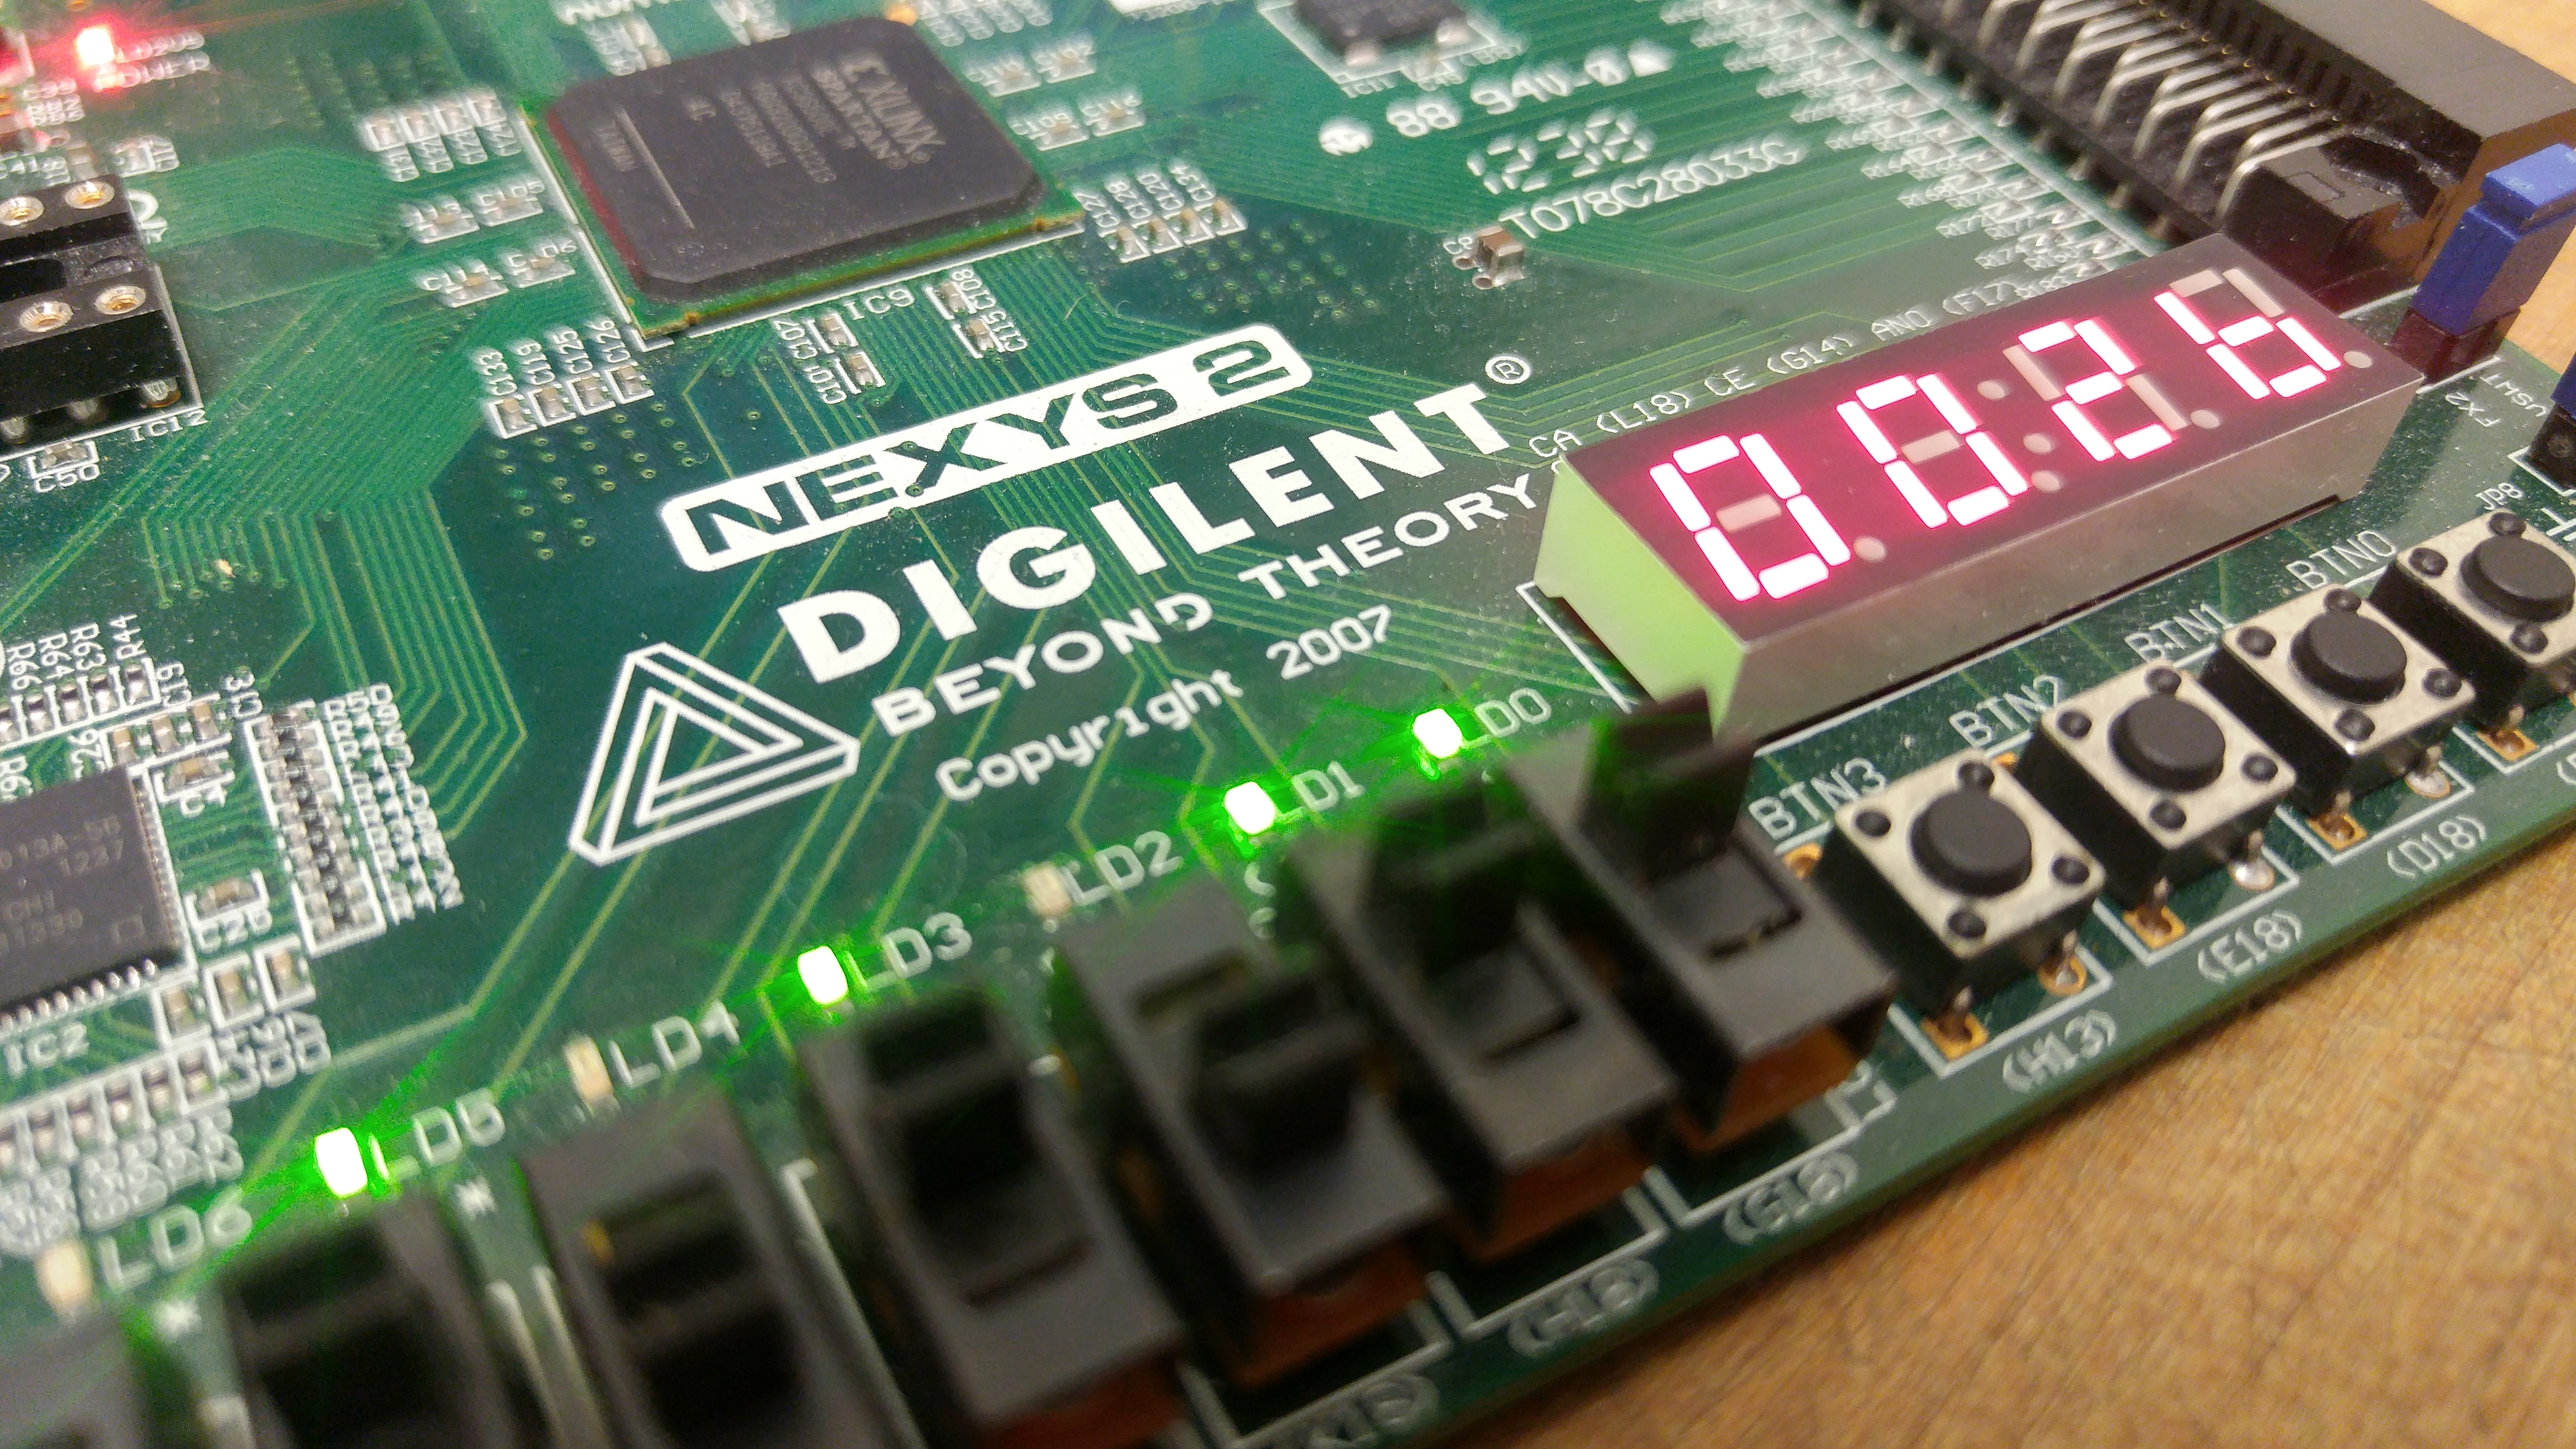
\includegraphics[width=0.45\textwidth]{pcb.jpg}
	\caption{Original image input to Sobel filter}
    \label{pcb-original}
\end{figure}
\begin{figure}[h]
	\centering
	\includegraphics[width=0.45\textwidth]{sobel_pcb.jpg}
	\caption{Magnitude of the gradient $||\boldsymbol{G}||$, as determined by applying a Sobel filter in both the $x$ and $y$ directions, at each pixel of the Gaussian-filtered original image with parameters $k = 5$ and $\sigma = 5$}
    \label{sobel-pcb}
\end{figure}
\begin{figure}[h]
	\centering
	\includegraphics[width=0.45\textwidth]{sobel_pcb_mesh.jpg}
	\caption{Gradient of Figure \ref{sobel-pcb} visualized as a three-dimensional mesh}
    \label{sobel-pcb-mesh}
\end{figure}

\subsection{Non-Maximum Suppression and Selective Thresholding}
Given the gradient magnitude and direction of the Gaussian-filtered image, the final step of the edge detection algorithm is to determine which pixels should be selected as edge pixels, and which should be rejected. We define two procedures, \textit{non-maximum suppression} and \textit{selective thresholding}, to gain a reasonably accurate edge map from the gradient.
\par Non-maximum suppression selects and rejects edge pixels according to the following criteria:
\begin{enumerate}
	\item Pixels whose gradient magnitude is below a user-defined low threshold, $t_l$, is immediately rejected
	\item If the gradient magnitude of a pixel is greater than that of the pixels in either direction of the gradient angle of that pixel, then the pixel is accepted if its gradient magnitude is greater than a user-defined high threshold, $t_h$
\end{enumerate}
More precisely, a pixel at $(i, j)$ with gradient magnitude $G_{i, j} > t_l$ and angle $\theta$ is accepted if any of the following hold true:
\begin{itemize}
	\item $(-\frac{\pi}{6} < \theta < \frac{\pi}{6} \vee -\pi < \theta < -\frac{5 \pi}{6} \vee \frac{5\pi}{6} < \theta < \pi) \wedge G_{i, j} > G_{i, j \pm 1}$
	\item $(\frac{\pi}{6} < \theta < \frac{\pi}{3} \vee -\frac{5 \pi}{6} < \theta < -\frac{2 \pi}{3}) \wedge G_{i, j} > G_{i \pm 1, \pm j}$
	\item $(\frac{\pi}{3} < \theta < \frac{2 \pi}{3} \vee -\frac{2 \pi}{3} < \theta < -\frac{\pi}{3}) \wedge G_{i, j} > G_{i \pm 1, j}$
	\item $(\frac{2 \pi}{3} < \theta < \frac{5 \pi}{6} \vee -\frac{\pi}{3} < \theta < -\frac{\pi}{6}) \wedge G_{i, j} > G_{i \pm 1, \mp j}$
\end{itemize}
The selective thresholding technique extends on the procedure of non-maximum suppression. For any pixel that passes crtiteria (2) (maximized, relative to the neighboring pixels, along the gradient direction), consider an $\alpha$ x $\alpha$ box around the pixel. If any pixel within the box exceeds the low threshold $t_l$, then the pixel is accepted. This technique attempts to catch pixels that might ``connect" ridge pixels identified by criteria (2) but fail to satify the criterion themselves, in order to create more continuous edge lines.
\begin{figure}[]
	\centering
	\includegraphics[width=0.45\textwidth]{pcb_edges.jpg}
	\caption{Output of edge detection algorithm after non-maximum suppression and selective thresholding on the image of Figure \ref{pcb-original}, with parameters $t_l = 70$ and $t_h = 80$}
    \label{pcb-edges}
\end{figure}
\begin{algorithm}[h]
	\smaller
	\label{non-maximum-suppression-selective-thresholding-algorithm}
	\caption{Non-maximum suppression and selective thresholding: pseudocode for a serial, CPU implementation}
	
	\KwIn{Gradient magnitude matrix $\boldsymbol{G}_{i, j}$ and gradient angle matrix $\boldsymbol{\theta}_{i, j}$ for an image $\boldsymbol{A}_{i, j}$, $\forall i \in [0, M - 1], \forall j \in [0, N - 1]$, $\alpha$ (representing the size of the box around which to apply selective thresholding), $t_h$ (the high threshold), and $t_l$ (the low threshold)}
	\KwOut{Edge matrix $\boldsymbol{E}$ of dimensions $M$ x $N$ that represent the edges of $\boldsymbol{A}$; any entry $\boldsymbol{E}_{i, j}$ is $255$ if an edge is present, and $0$ if an edge is not present}
	
	\nl Initialize $\boldsymbol{E}$ to 0 $\forall i \in [0, M - 1], \forall j \in [0, N - 1]$\;
	\nl \ForEach {$i \in [\alpha + 1, M - \alpha - 2]$} {
		\nl \ForEach {$j \in [\alpha + 1, N - \alpha - 2]$} {
			\nl HorizontalGradient $\gets -\frac{\pi}{6} < \boldsymbol{\theta}_{i, j} < \frac{\pi}{6} \vee -\pi < \boldsymbol{\theta}_{i, j} < -\frac{5 \pi}{6} \vee \frac{5\pi}{6} < \boldsymbol{\theta}_{i, j} < \pi$\;
			\nl HorizontalMax $\gets$ HorizontalGradient $\wedge \boldsymbol{G}_{i, j} > \boldsymbol{G}_{i, j \pm 1}$\;
			\nl PosDiagonalGradient $\gets \frac{\pi}{6} < \boldsymbol{\theta}_{i, j} < \frac{\pi}{3} \vee -\frac{5 \pi}{6} < \boldsymbol{\theta}_{i, j} < -\frac{2 \pi}{3}$\;
			\nl PosDiagonalMax $\gets$ PosDiagonalGradient $\wedge \boldsymbol{G}_{i, j} > \boldsymbol{G}_{i \pm 1, \pm j}$\;
			\nl VerticalGradient $\gets \frac{\pi}{3} < \boldsymbol{\theta}_{i, j} < \frac{2 \pi}{3} \vee -\frac{2 \pi}{3} < \boldsymbol{\theta}_{i, j} < -\frac{\pi}{3}$\;
			\nl VerticalMax $\gets$ VerticalGradient $\wedge \boldsymbol{G}_{i, j} > \boldsymbol{G}_{i \pm 1, j}$\;
			\nl NegDiagonalGradient $\gets \frac{2 \pi}{3} < \boldsymbol{\theta}_{i, j} < \frac{5 \pi}{6} \vee -\frac{\pi}{3} < \boldsymbol{\theta}_{i, j} < -\frac{\pi}{6}$\;
			\nl NegDiagonalMax $\gets$ NegDiagonalGradient $\wedge \boldsymbol{G}_{i, j} > \boldsymbol{G}_{i \pm 1, \mp j}$\;
			
			\nl \If {$\boldsymbol{G}_{i, j} > t_h \wedge ($\textnormal{HorizontalMax} $\vee$ \textnormal{PosDiagonalMax} $\vee$ \textnormal{VerticalMax} $\vee$ \textnormal{NegDiagonalMax}$)$} {
				\ForEach {$i' \in [-\alpha, \alpha]$} {
					\ForEach {$j' \in [-\alpha, \alpha]$} {
						\nl \If{$\boldsymbol{G}_{i + i', j + j'} > t_l$} {
							\nl $\boldsymbol{E}_{i + i', j + j'} \gets 255$\;
						}
					}
				}
			}
		}
	}
	\nl \Return $\boldsymbol{E}$\;
	\
\end{algorithm}

\subsection{GPU Parallelization and CUDA Implementation}
We begin with a parallelized implementation of separable convolution, since the same operation is applied for both the initial Gaussian low pass filter


\section{Motion Detection Algorithm}
Our motion detection algorithm compares the edges from two frames temporally separated by a small interval of time and attempts to estimate regions of the frame that exhibit movement or motion. This process is then repeated continuously to provide a real-time visualization of the regions of movement in a continuous video stream. The motion detection algorithm we present is composed of the following steps:
\begin{enumerate}
	\item Given two frames $\boldsymbol{F}_1$ and $\boldsymbol{F}_2$ separated by a time interval of $\Delta t$, compute its edges $\boldsymbol{E}_1$ and $\boldsymbol{E}_2$.
	\item Create a strict binary difference matrix $\boldsymbol{D}_0$ between $\boldsymbol{E}_1$ and $\boldsymbol{E}_2$ whose value is high at locations at which an edge is present in frame but not the other, and low at locations at which both frames have an edge or no edge.
	\item Apply a parameter-controlled movement tolerance thresholding operation to the matrix $\boldsymbol{D}_0$ to obtain matrix $\boldsymbol{D}$, in order to suppress potential false positives of detected motion from incidental camera movement.
\end{enumerate}
\par $\boldsymbol{F}_1$ and $\boldsymbol{F}_2$ are obtained by sampling frames from a continuous video stream, a task aided by the OpenCV C library. Thus, the time interval $\Delta t$ will be small enough for a real-time algorithm. The edges $\boldsymbol{E}_1$ and $\boldsymbol{E}_2$ are computed with the edge detection algorithm of Section II. Below, we explore, in greater depth, the procedures for building a thresholded diffrence matrix and finally estimating the motion area by analyzing a spatial difference density map.

\subsection{Thresholded Frame-by-Frame Difference Map}
The preliminary requirement in determining areas of motion from two frames is a systematic method of determining and quantifying the differences between two frames separated by a small $\Delta t$. Intuitively, areas of motion within the time interval $\Delta t$ should exist at locations at which the difference between the two frames is large. This process is then continuously repeated for every pair of input frames in order to create a real-time motion detector. In our algorithm, we quantify differences on a binary basis using edge data from our edge detection algorithm, then determine motion locations from a thresholded density map of the difference matrix $\boldsymbol{D}$.
\par More formally, we begin with a matrix $\boldsymbol{D}_0$ created from a simple comparison of $\boldsymbol{E}_1$ and $\boldsymbol{E}_2$.
\[
\boldsymbol{D}_0 = |\boldsymbol{E}_1 - \boldsymbol{E}_2| =
\begin{cases}
	255 & \boldsymbol{E}_{1_{i, j}} \neq \boldsymbol{E}_{2_{i, j}} \\
	0 & \boldsymbol{E}_{1_{i, j}} = \boldsymbol{E}_{2_{i, j}}
\end{cases}
\]
Then, for each location $(i, j)$ in $\boldsymbol{D}_0$, a thresholded difference matrix $\boldsymbol{D}$ is created by considering a box of constant size $\beta$ x $\beta$ around that pixel and suppressing the value of the surrounding pixels to 0 if its value matches that at $\boldsymbol{D}_{0_{i, j}}$. This step is designed to reduce false positives of motion detection arising from stray movement of the frame (e.g. camera shake). The computation of $\boldsymbol{D}$ is demonstrated in Algorithm \ref{difference-matrix-algorithm}. The output matrix is then used as input to building a spatial difference density map, from which we estimate motion locations.
\begin{figure}[H]
	\centering
	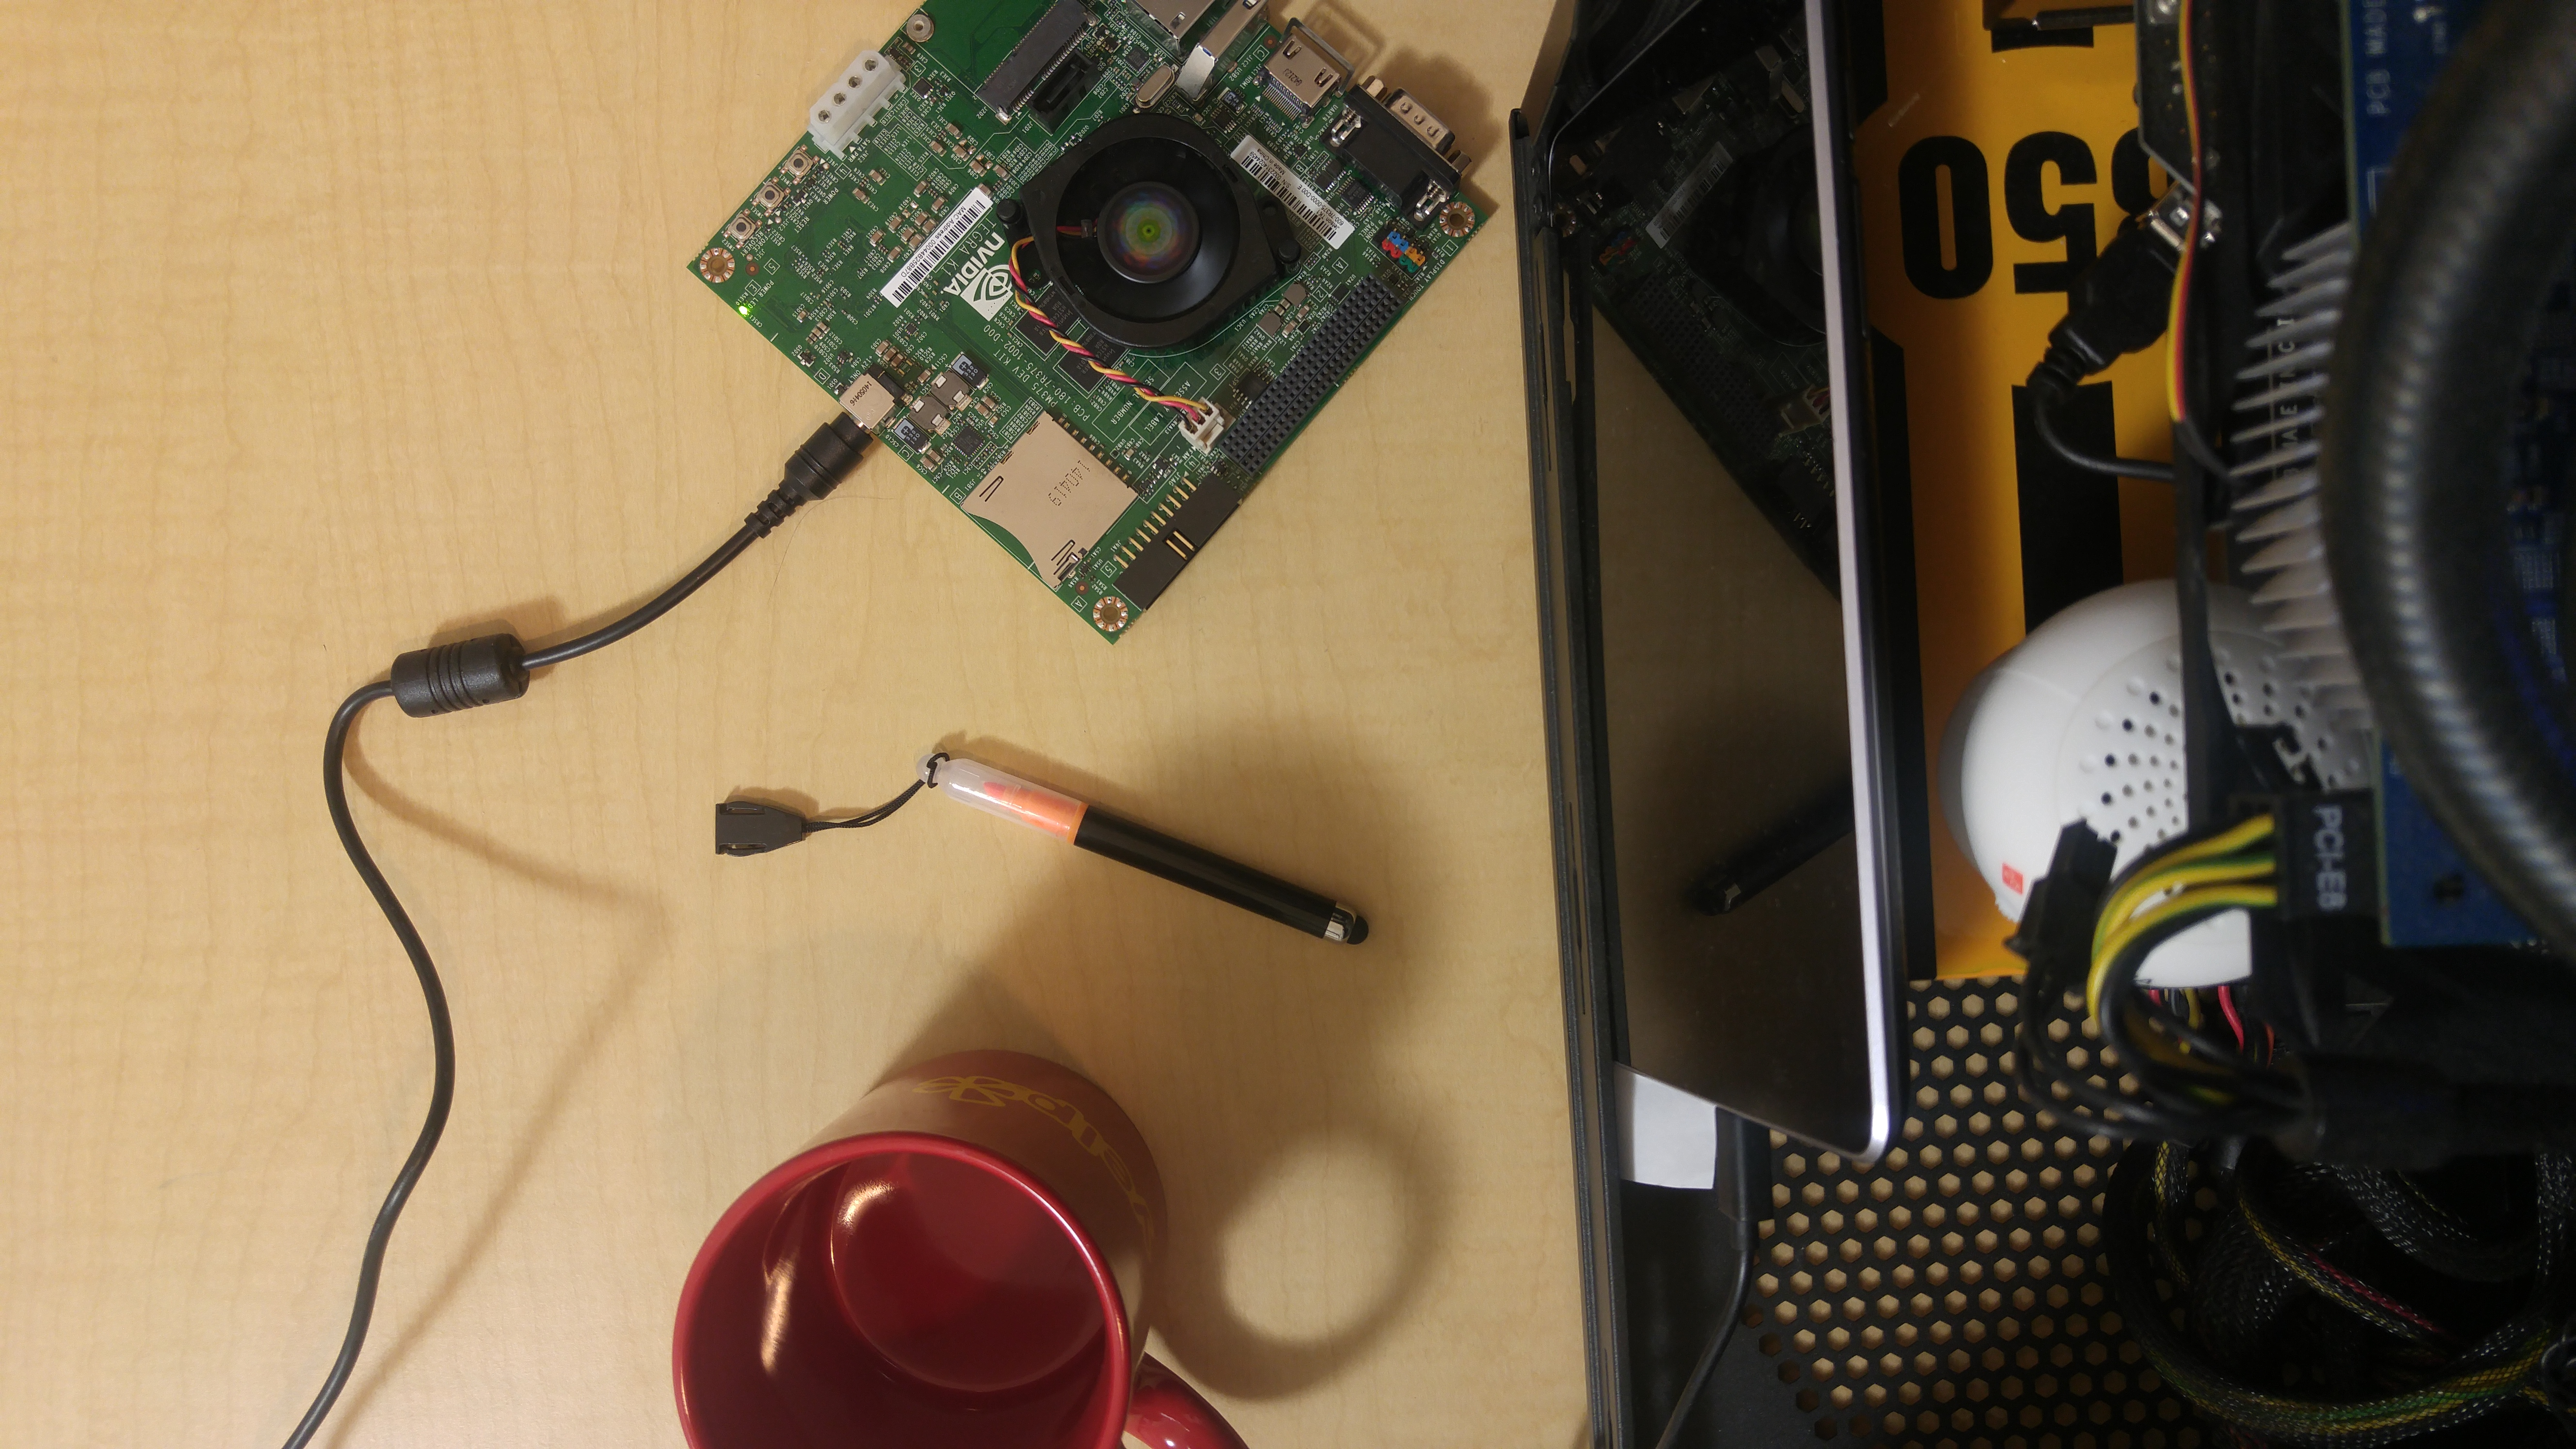
\includegraphics[width=0.45\textwidth]{desk_1.jpg}
	\caption{Example of difference matrix computation: original initial frame $\boldsymbol{F}_1$ of dimensions $5312$ x $2988$}
    \label{desk-1-original}
\end{figure}
\begin{figure}[H]
	\centering
	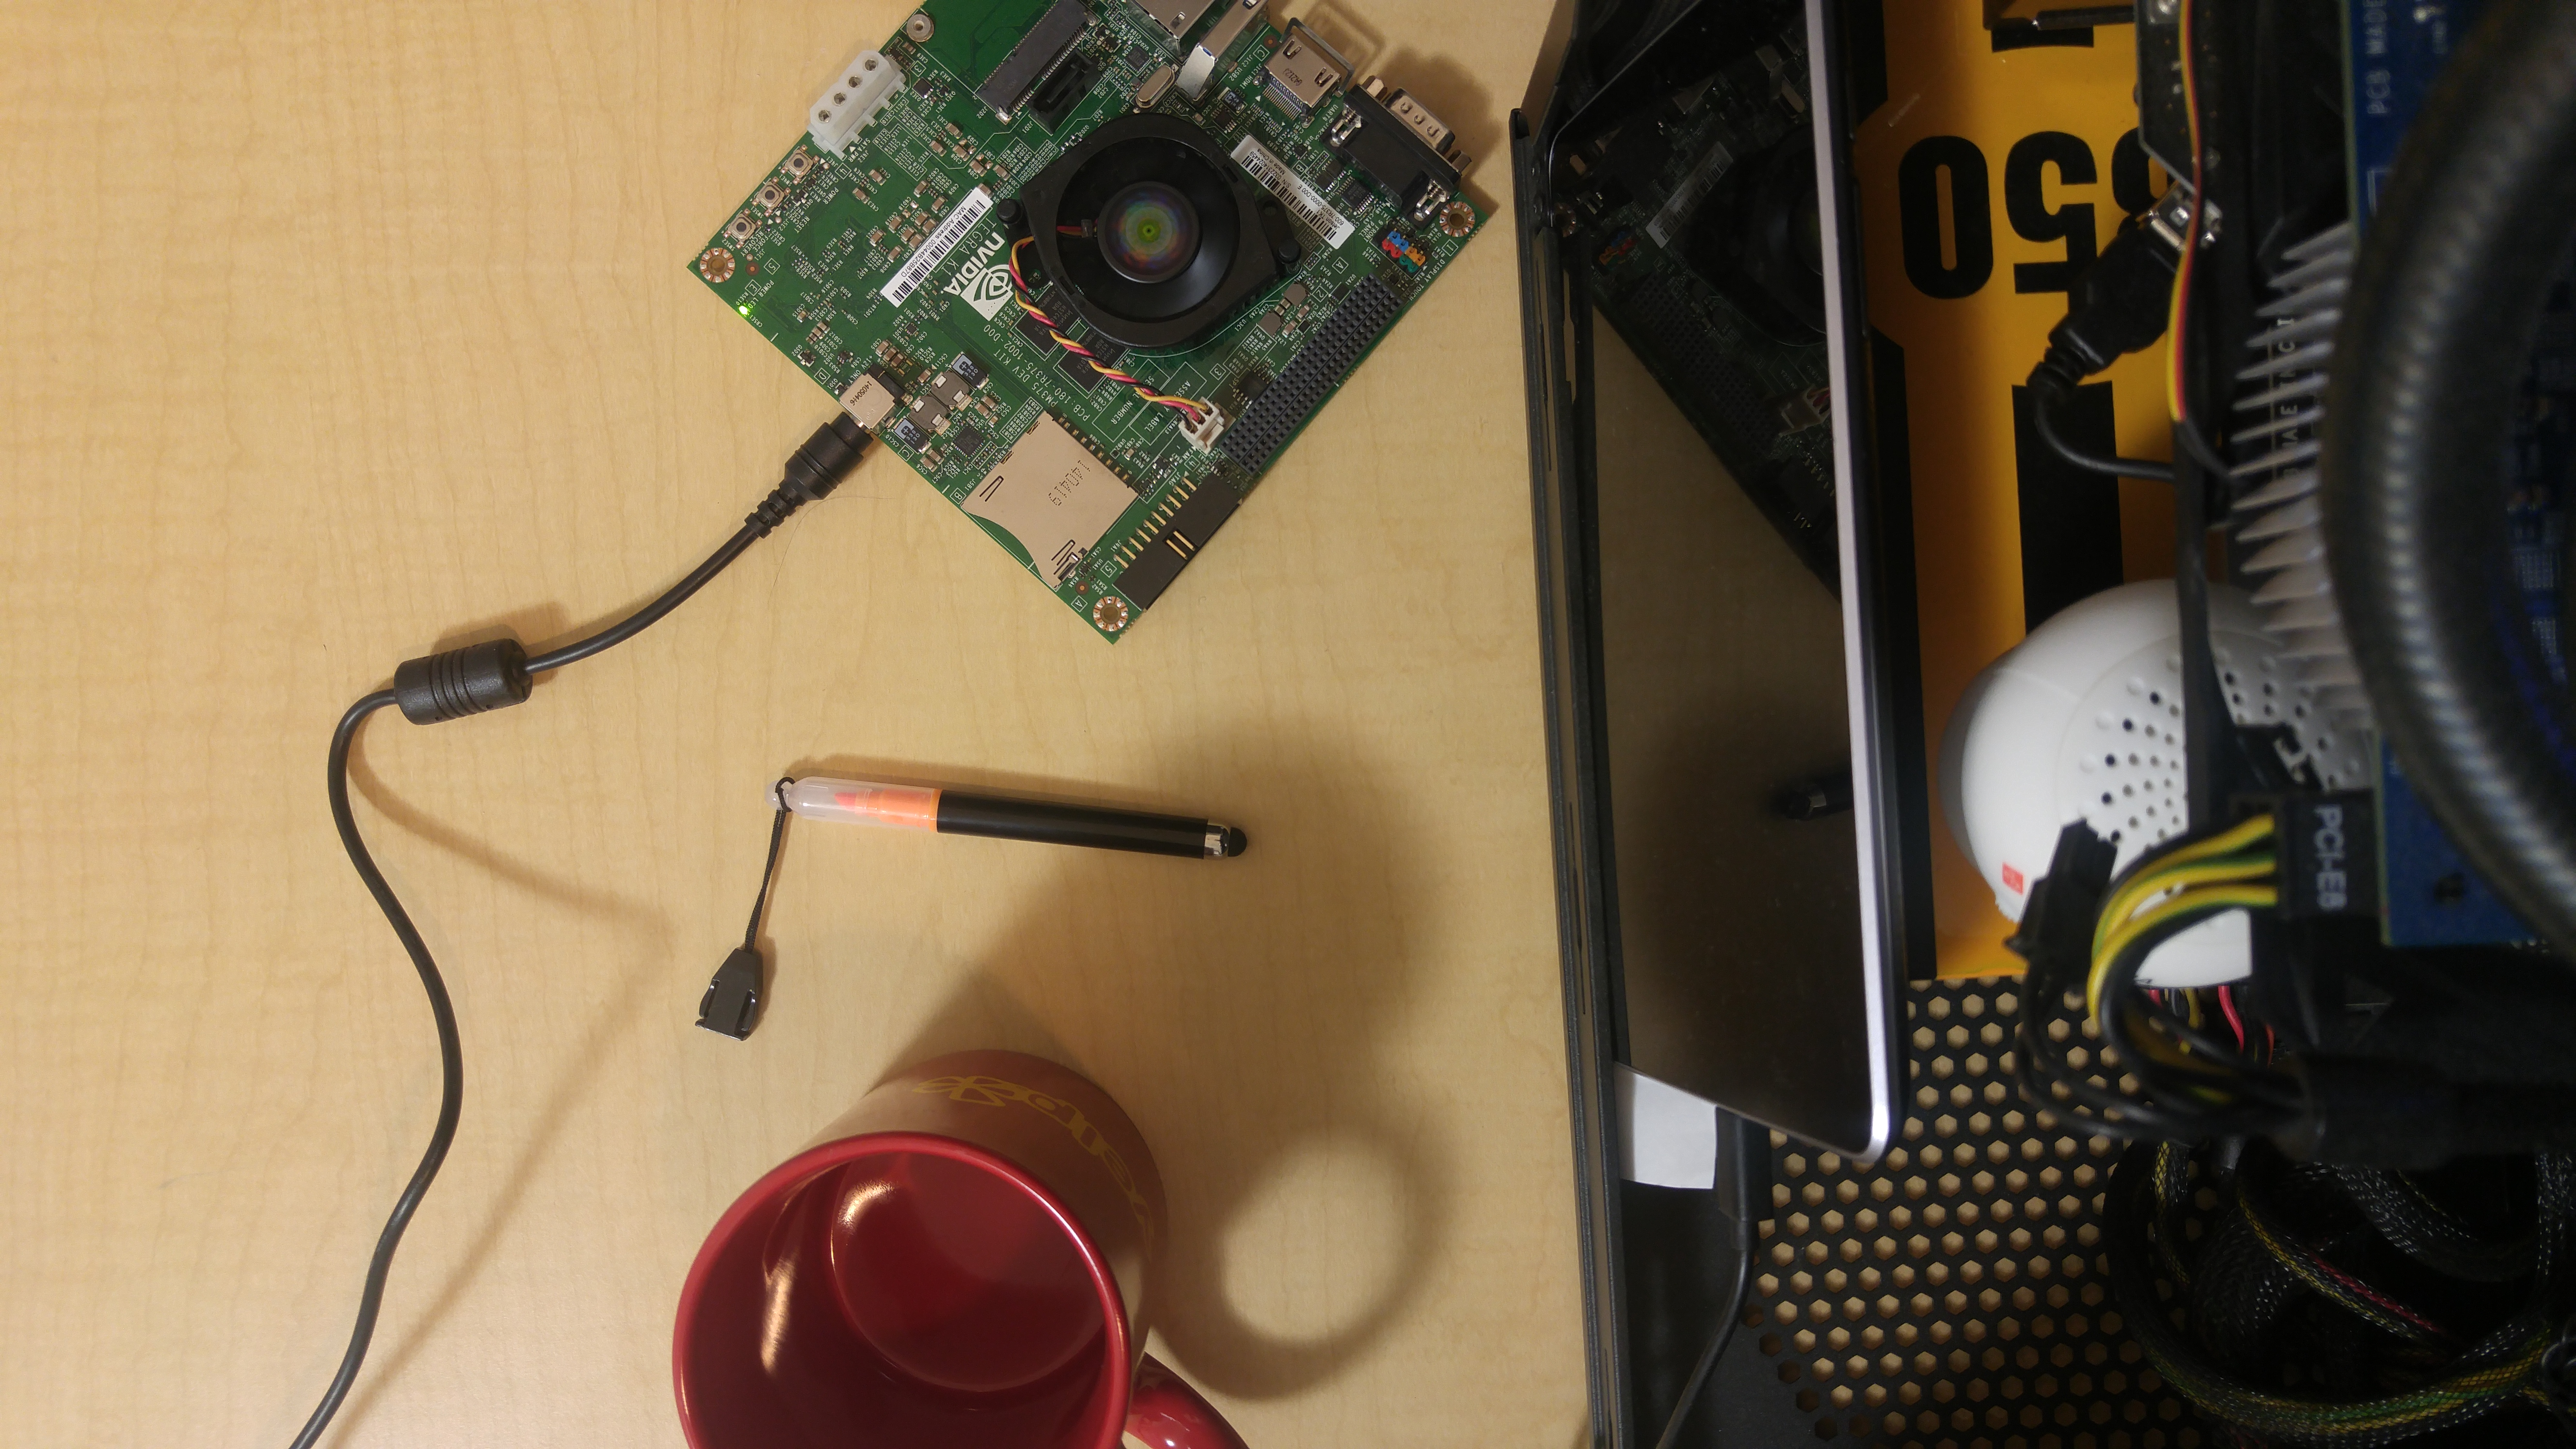
\includegraphics[width=0.45\textwidth]{desk_2.jpg}
	\caption{Example of difference matrix computation: original initial frame $\boldsymbol{F}_2$ (the item displaced between the two frames is the highlighter at the center)}
    \label{desk-2-original}
\end{figure}
\begin{figure}[H]
	\centering
	\includegraphics[width=0.45\textwidth]{desk_edges_1.jpg}
	\caption{Example of difference matrix computation: edges of the initial frame $\boldsymbol{E}_1$ computed with parameters $k = 5$, $\sigma = 5$, $t_l = 15$, $t_h = 25$}
    \label{desk-1-edges}
\end{figure}
\begin{figure}[H]
	\centering
	\includegraphics[width=0.45\textwidth]{desk_edges_2.jpg}
	\caption{Example of difference matrix computation: edges of the initial frame $\boldsymbol{E}_2$ computed with parameters $k = 5$, $\sigma = 5$, $t_l = 15$, $t_h = 25$}
    \label{desk-2-edges}
\end{figure}
\begin{figure}[H]
	\centering
	\includegraphics[width=0.45\textwidth]{desk_difference.jpg}
	\caption{Example of difference matrix computation: difference matrix $\boldsymbol{D}$ with parameter $\beta = 12$}
    \label{desk-difference}
\end{figure}
\begin{algorithm}[]
	\smaller
	\label{difference-matrix-algorithm}
	\caption{Determining the difference matrix between two frames, given their edge data: pseudocode for a serial, CPU implementation}
	
	\KwIn{Edge matrices $\boldsymbol{E}_1$ and $\boldsymbol{E}_2$, both of dimensions $M$ x $N$, and movement tolerance threshold $\beta$}
	\KwOut{Thresholded difference matrix $\boldsymbol{D}$; any entry $\boldsymbol{D}_{i, j}$ is $255$ if there is a difference, $0$ otherwise}
	
	\nl Initialize $\boldsymbol{D}_{i, j}$ to 0 $\forall i \in [0, M - 1], \forall j \in [0, N - 1]$\;
	\nl \ForEach {$i \in [0, M - 1]$} {
		\nl \ForEach {$j \in [0, N - 1]$} {
			\nl \If {$\boldsymbol{E}_{1_{i, j}} \neq \boldsymbol{E}_{2_{i, j}}$} {
				\nl $\boldsymbol{D}_{i, j} \gets 255$\;
				\ForEach {$i' \in [-\beta, \beta]$} {
					\ForEach {$j' \in [-\beta, \beta]$} {
						\nl \If{$(i + i', j + j')$ \textnormal{is within the bounds of} $E_1$ \textnormal{and} $\boldsymbol{E}_{1_{i + i', j + j'}} = \boldsymbol{E}_{2_{i + i', j + j'}}$} {
							\nl $\boldsymbol{D}_{i + i', j + j'} \gets 0$\;
						}
					}
				}
			}
		}
	}
	\nl \Return $\boldsymbol{D}$\;
	\
\end{algorithm}


\subsection{Motion Area Estimation via a Spatial Difference Density Map}
The difference matrix $\boldsymbol{D}$ determined with Algorithm \ref{difference-matrix-algorithm} is effectively a maximally precise estimate of motion area (e.g., to the resolution of a single pixel, since $\boldsymbol{D}$ is computed on a pixel-by-pixel basis). However, in practice, it is more useful to consider general regions of the image around which motion exists. For this reason, we build a density map of the matrix $\boldsymbol{D}$ using equal-sized rectangular sections of the input image that approximates the density of the difference per unit area (units pixels$^2$). Thus, the original $M$ x $N$ difference matrix $\boldsymbol{D}$ is reduced to a matrix $\boldsymbol{D}'$ of size $m$ x $n$ such that
$$M = k_1 m$$
$$N = k_2 n$$
where $k_1, k_2 \in \mathbb{Z}$. Intuitively, choosing a higher $k_1$ and $k_2$ will result in a higher resolution over which the density is evaluated. Selection of $k_1$ and $k_2$ should depend on how large of a region over which motion should be estimated. The upper limits of $k_1$ and $k_2$ are $M$ and $N$, respectively, at which point $\boldsymbol{D}'$ = $\boldsymbol{D}$. Each index $(m, n)$ in $\boldsymbol{D}'$ corresponds to the upper-left corner of a rectangular section of $\boldsymbol{A}$ whose width is $\frac{M}{m}$ and height is $\frac{N}{n}$.
\par Regions of motion are the rectangular sections whose density exceeds a user-defined threshold $\Gamma$, denoting the number of difference pixels over the total number of pixels considered in the rectangular section. For each such region $\boldsymbol{R}$ in $\boldsymbol{A}$ of size $\frac{M}{m}$ x $\frac{N}{n}$,
$$\textnormal{DifferenceDensity}(\boldsymbol{R}) = \frac{\textnormal{number of pixel differences in } \boldsymbol{R}}{\textnormal{number of pixels in } \boldsymbol{R}}$$
\[
\boldsymbol{D}' =
\begin{cases}
1 & \textnormal{DifferenceDensity}(\boldsymbol{R}) > \Gamma\\
0 & \textnormal{otherwise}
\end{cases}
\]
\begin{algorithm}[]
	\smaller
	\label{difference-density-matrix-algorithm}
	\caption{Estimating regions of motion in an image with a difference density matrix: pseudocode for a serial, CPU implementation}
	
	\KwIn{Thresholded difference matrix $\boldsymbol{D}$, motion threshold $\Gamma$, width of the original image $M$, height of the original image $N$, number of horizontal divisions $m$, and number of vertical divisions $n$}
	\KwOut{The difference density matrix $\boldsymbol{D}'$ of dimensions $m$ x $n$ whose value is 1 if there is motion in that region, and 0 otherwise}
	
	\nl Initialize $\boldsymbol{D}'$ to 0 $\forall i \in [0, m - 1], \forall j \in [0, n - 1]$\;
	\nl \ForEach {$i \in [0, m - 1]$} {
		\nl \ForEach {$j \in [0, n - 1]$} {
			\nl $x \gets 0$\tcp*{Number of differences in this region}
			\nl \ForEach{$i' \in [0, \frac{M}{n}]$} {
				\nl \ForEach{$j' \in [0, \frac{N}{n}]$} {
					\nl \If {$\boldsymbol{D}_{i + i', j + j'} \neq 0$} {
						\nl $x \gets x + 1$\;
					}
				}
			}
			\nl \If{$\frac{mn}{MN}x > \Gamma$} {
				\nl $\boldsymbol{D}'_{i, j} \gets 1$\;
			}
		}
	}
	\nl \Return $\boldsymbol{D}'$\;
	\
\end{algorithm}


\section{GPU Speedup Results}
Placeholder text


\section{Conclusion}
Placeholder text

\section*{Acknowledgments}
Placeholder text

\end{document}